\documentclass[a4paper]{article}
\usepackage{pdfpages, pgffor}
\setlength{\fboxrule}{0.3mm}

\begin{document}
\newwrite\myoutput
\immediate\openout\myoutput=\jobname.options
\immediate\write\myoutput{\unexpanded{\documentclass[10pt, handout, aspectratio=169]{beamer}}} %43 for 4x3, 169 for 16x9, 1610 for 16x10
\immediate\closeout\myoutput
\foreach \n in {1,...,8}{
    \IfFileExists{week\n/week\n.tex}{
        \immediate\write18{texify.exe --pdf  --clean week\n/week\n.tex}
        \includepdf[pages=-,nup=2x2,delta=5pt 30pt,landscape=true,frame=true,column=false,noautoscale=false]{week\n.pdf}
    }
}
\end{document}

\usetheme{Frankfurt}
\usecolortheme{crane}

\usepackage{exscale,latexsym,microtype,amsmath,amssymb,amsfonts,graphicx,natbib,times,booktabs,xstring}

\newcommand{\E}{\ensuremath{{\mathbb E}}} % expected value
\newcommand{\R}{\ensuremath{{\mathbb R}}}
\newcommand{\Var}{\ensuremath{{\mathbb V}}} % variance
\newcommand{\frameit}[2]{\begin{frame}\frametitle{#1}\begin{itemize}#2\end{itemize}\end{frame}}
\def\func#1{\mathop{\rm #1}}
\def\er#1{\emph{\color{red}#1}}
\def\newblock{\hskip .11em plus .33em minus .07em}
\def\limfunc#1{\mathop{\rm #1}}%
\setbeamertemplate{blocks}[rounded][shadow=true]
\date{}

\titlegraphic{
\includegraphics[height =0.4in]{../HSLU_Logo_EN_Schwarz_rgb}}
\title{Module 9.3: Time Series Analysis with Python\\Fall Term\space\number\year}
\def\theweek{\StrRight{\jobname}{1}}
\author[Week \theweek]{\textbf{Week \theweek}:}
\AtBeginSection{
\frame{
\frametitle{Outline}
\tableofcontents[currentsection]
}}


\institute{{\Large Introduction; Descriptive Time Series Analysis}}
\begin{document}
\frame{\titlepage}
\begin{frame}%
\frametitle{Outline in Weeks}
\begin{enumerate}
\item Introduction; Descriptive Modeling
\item Returns; Autocorrelation; Stationarity
\item ARMA Models
\item Unit Roots; ARIMA Models
\item Volatility Modeling
\item Value at Risk
\item Cointegration
%\item Panel Data
\end{enumerate}
\end{frame}% 

\section{Preliminaries}\subsection*{bla}
\begin{frame}
\frametitle{General Information}
\begin{itemize}
\item Lectures will be a mix of theory and practice.
\item Slides and additional materials are available on Ilias.
\item 90 min.\ written exam during exam phase, closed book. Details will be communicated later.
\item A mock exam will be made available.
\end{itemize}
\end{frame}
\begin{frame}
\frametitle{Book}
\begin{itemize}
\item Course is not explicitly based on any book.
\item If you prefer to have a book, then I recommend Brooks (2019)\footnote{Brooks, C. (2019). Introductory Econometrics for Finance (4th ed.). Cambridge: Cambridge University Press.}. A reading list follows on the next slide.
\item I will also make selected problems and solutions available.
\end{itemize}
\end{frame}
\begin{frame}
\frametitle{Reading List: Brooks (2019)}

\begin{enumerate}
\item[Pre] As a refresher, Sections 1.1--1.6 (mathematical foundations), 2.1--2.7 (statistics and distribution theory).
\item[Week 1] (not covered in book)
\item[Week 2] Sections 6.1 and 6.2
\item[Week 3] Sections 6.3--6.10
\item[Week 4] Section 8.1; Section 5.5
\item[Week 5] Sections 9.1--9.16; 9.17
\item[Week 6] (not covered in book)
\item[Week 7] Sections 8.3 -- 8.11
\item[Week 7] Sections 11.1--11.7; Section 14.2

\end{enumerate}
\end{frame}
\section{Introduction}\subsection*{bla}
\frameit{What is Time Series Analysis}{
\item In Module 9.2, you learned about the classical linear regression model (\er{CLRM}).
\item It is used to estimate linear relationships of the form
\[
Y_i=\beta_0+\beta_1x_{i}+U_i\tag{\dag}\label{csr},
\]
possibly with more than one regressor.
\item Typically, 5 assumption are made about the error term: zero mean, constant variance (homoskedasticity), lack of autocorrelation, no correlation with the regressors (orthogonality), normality.
\item These are often justifiable for \er{cross-sectional} data, where each observation $i$ corresponds to a different entity (e.g., a firm, a country, etc.).
}
\frameit{What is Time Series Analysis}{
\item In many areas of financial econometrics (risk models, asset pricing, ...), one deals with \er{time series data} instead; here, every observation corresponds to a different \er{time period}. Examples:
\begin{itemize}
\item the price of IBM stock on each trading day since Jan 2nd, 2004;
\item monthly inflation in the EUR area since Jan 2002;
\item US GDP growth in every quarter since 1986Q1, etc.
\end{itemize}
\item As seen above, time series may have different \er{frequencies} (daily, monthly, quarterly, etc.).
\item We will only cover \er{regular} time series: observations occur at equally spaced time points (e.g., daily closing prices for stocks).
}
\frameit{What is Time Series Analysis}{
\item To highlight the fact that we are dealing with time series, we use a subscript $t$ instead of $i$; thus, a regression model such as \ref{csr} would be written
\[
Y_t=\beta_0+\beta_1x_{t}+U_t\tag{\ddag}\label{tsr}
\]
if $\{Y_t\}$ and $\{x_t\}$ are time series.

\item Regression \ref{tsr} is unlikely to satisfy the CLRM assumtions; time series usually exhibit \er{autocorrelation}, and often changes in standard deviation (or in ``volatility'', for stock returns).
\item Time series analysis is the study of methods to deal with these salient features.
\item The broader goal (as usual in econometrics) is to empirically \er{verify} economic theories (e.g., the CAPM).
\item Another important aspect is \er{forecasting} (e.g, GDP forecasts, inflation forecasts, Value at Risk forecasts, etc.)
}
\frameit{What is Time Series Analysis}{
\item For most of the course, we will consider \er{univariate} time series analysis.
\item This means that instead of a regression like
\[
Y_t=\beta_0+\beta_1x_{t}+U_t
\]
above, we only have \er{one} time series $\{Y_t\}$.
\item The goal is to describe the (dynamic) behavior of $Y_t$, e.g., for forecasting.
\item We'll start with a purely \er{descriptive} approach today. Starting next week, we'll move on to actual dynamic models.
}
\section{Examples}\subsection*{bla}
\frame{
\begin{block}{Bitcoin prices}
\begin{center}
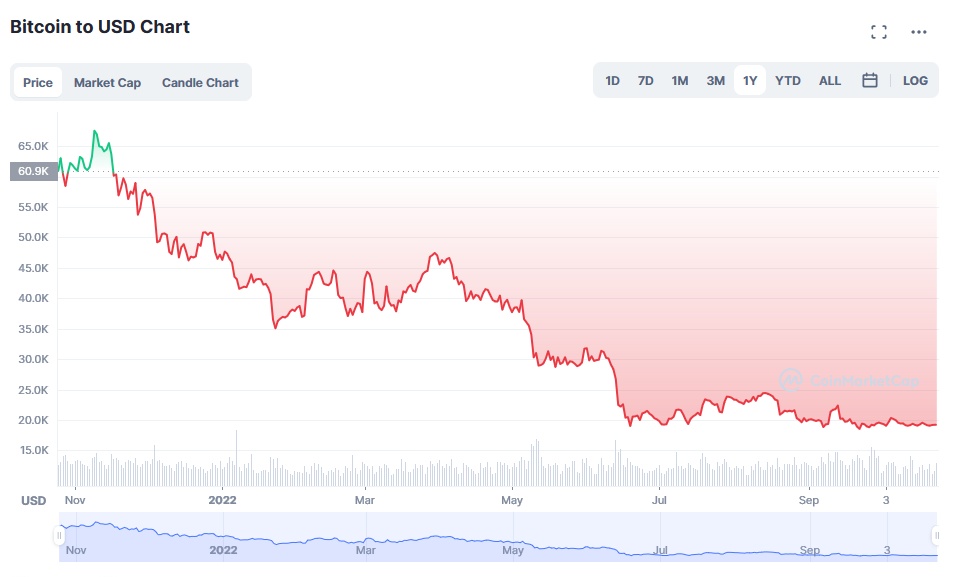
\includegraphics[width=0.8\textwidth]{btc.png}
\end{center}
\footnotesize{Source: \href{https://coinmarketcap.com/currencies/bitcoin/}{\color{blue}coinmarketcap.com}}
\end{block}
}
\frame{
\begin{block}{CoViD19 Hospitalizations}
\begin{center}
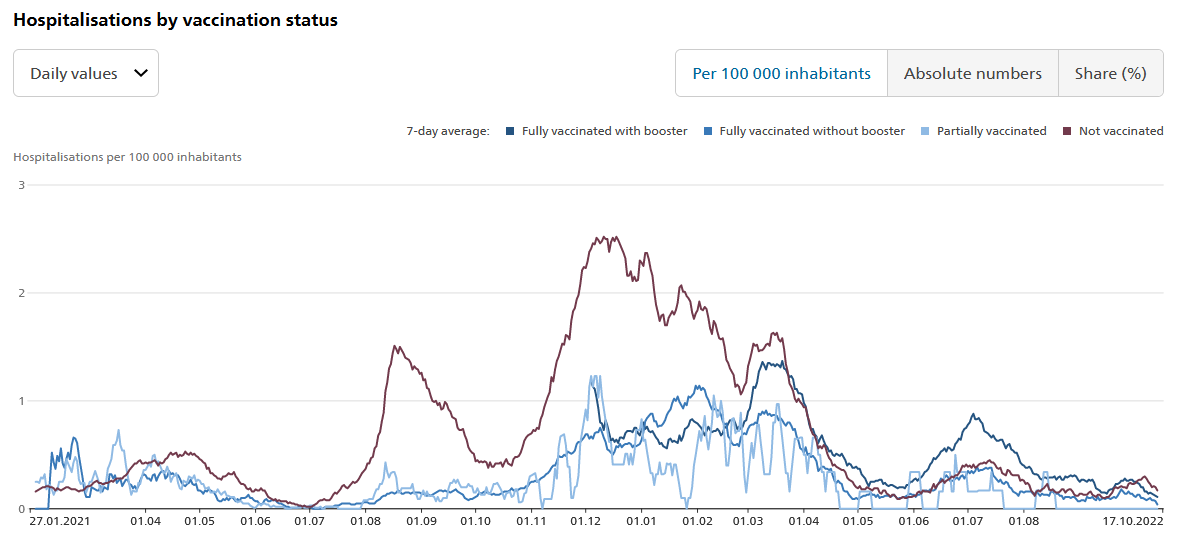
\includegraphics[width=0.8\textwidth]{covid.png}
\end{center}
\footnotesize{Source: \href{https://www.covid19.admin.ch/en/vaccination/status?vaccStatusDevRel=inz100k}{\color{blue}covid19.admin.ch}}
\end{block}
}
\frame{
\begin{block}{Tesla Stock}
\begin{center}
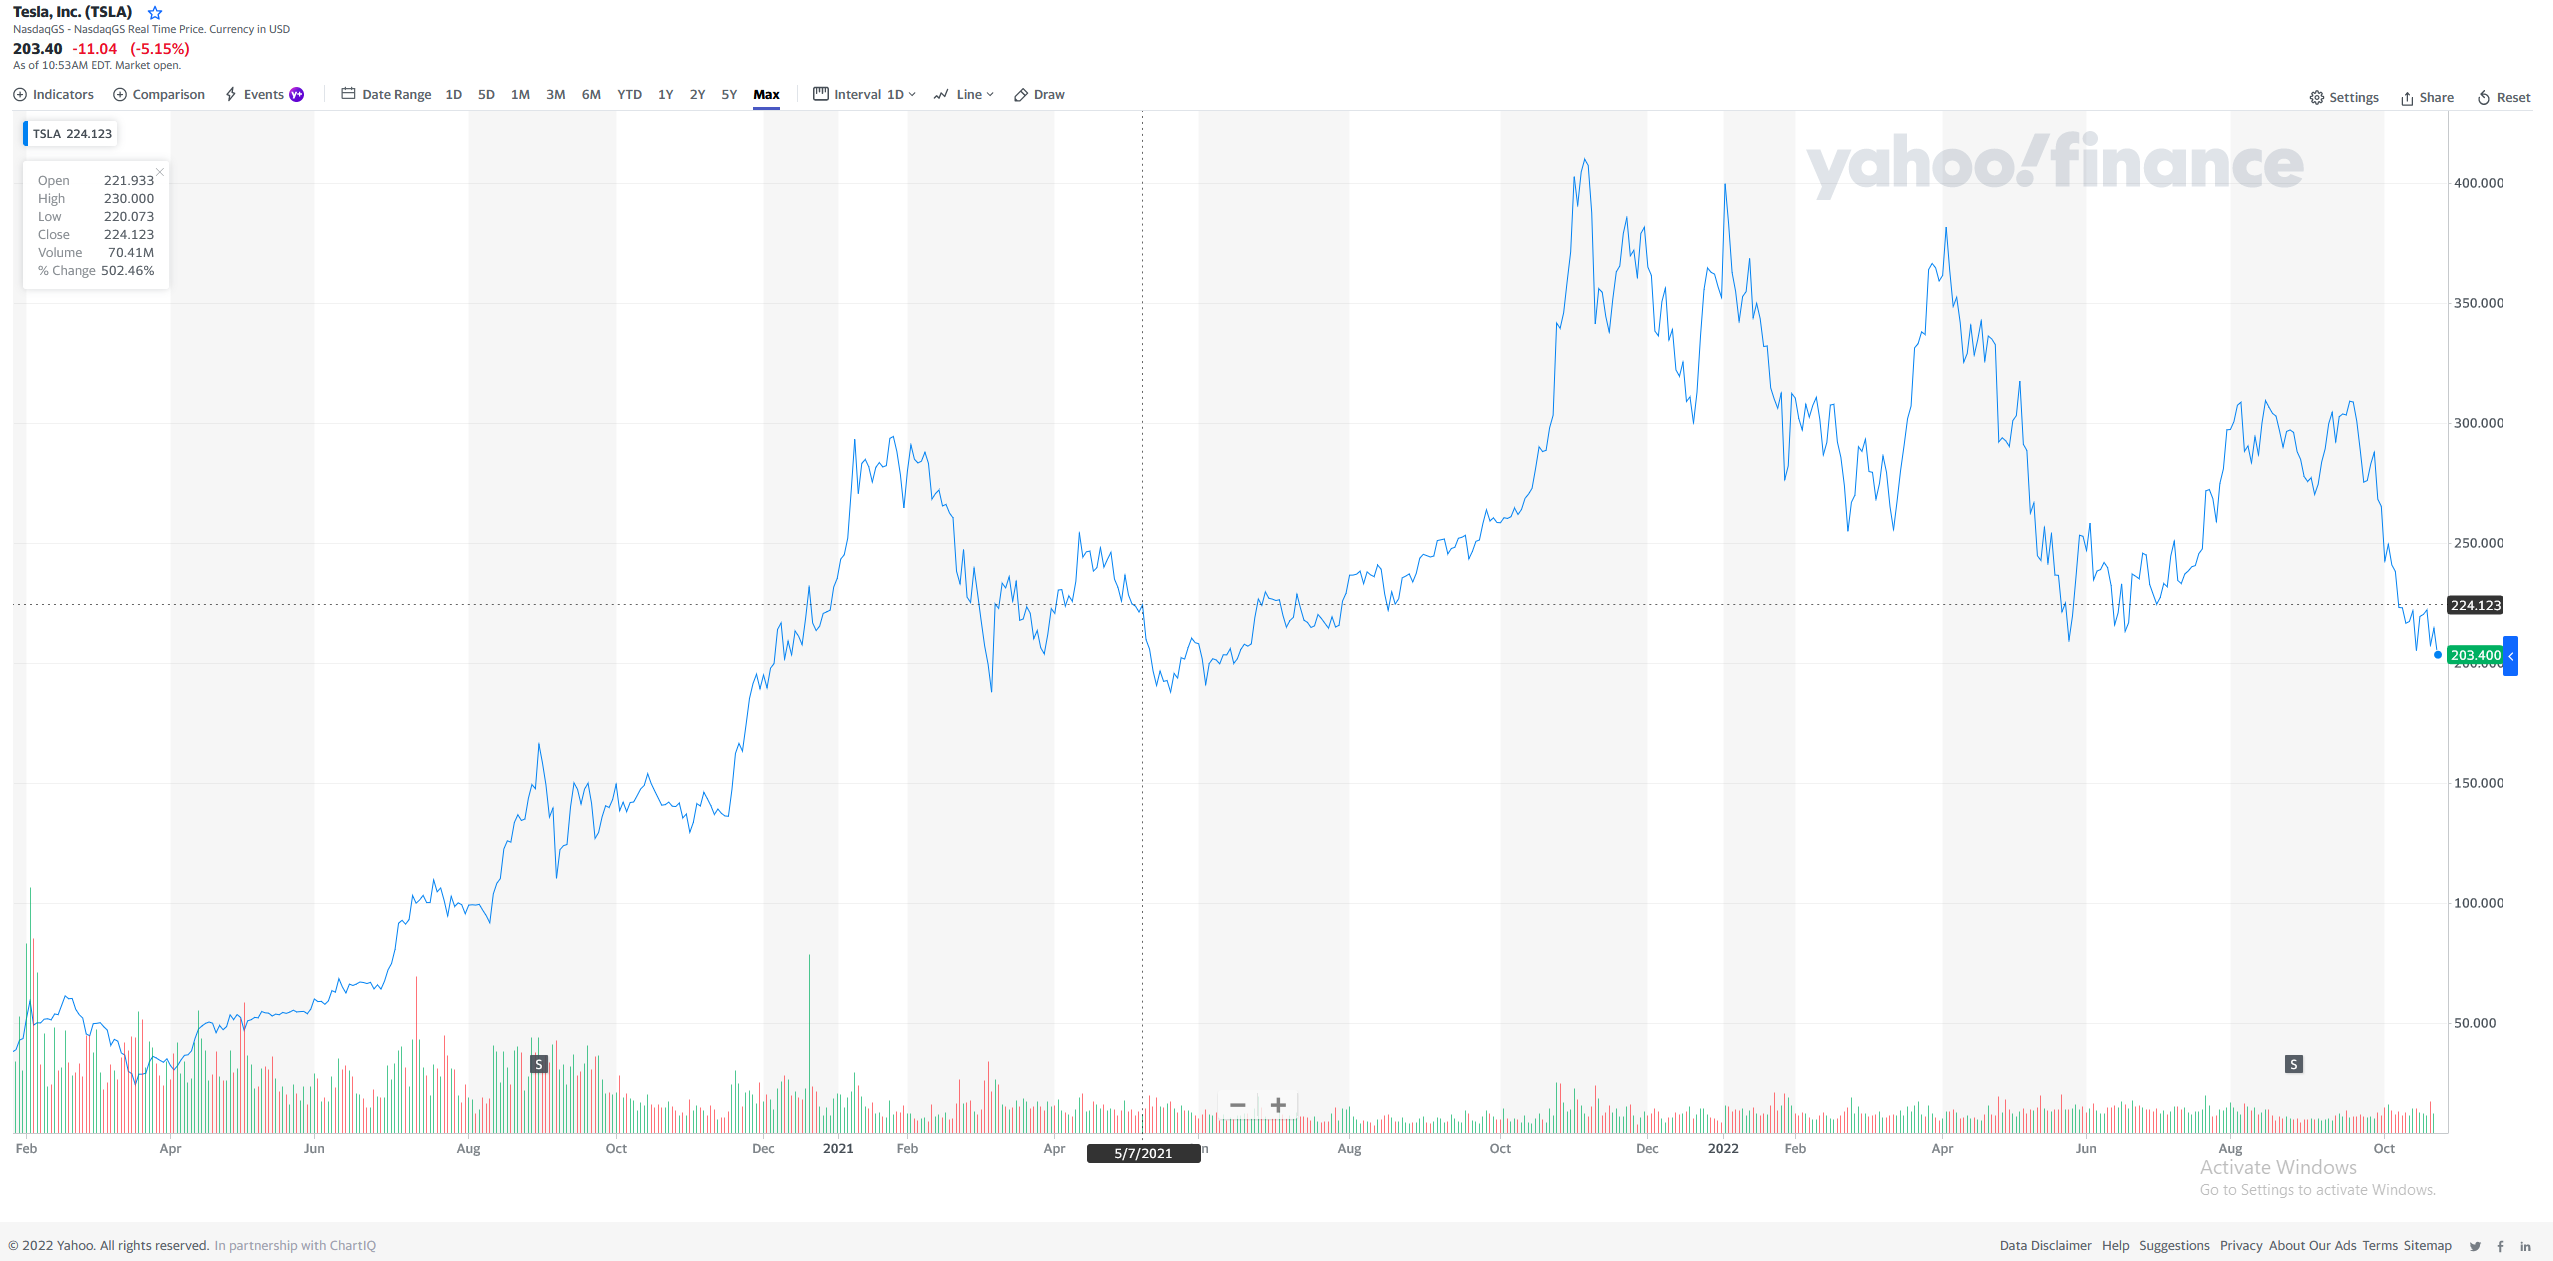
\includegraphics[width=0.8\textwidth]{tesla.png}
\end{center}
\footnotesize{Source: \href{https://finance.yahoo.com/quote/TSLA/}{\color{blue}Yahoo Finance}}
\end{block}
}
\frame{
\begin{block}{Unemployment in Switzerland}
\begin{center}
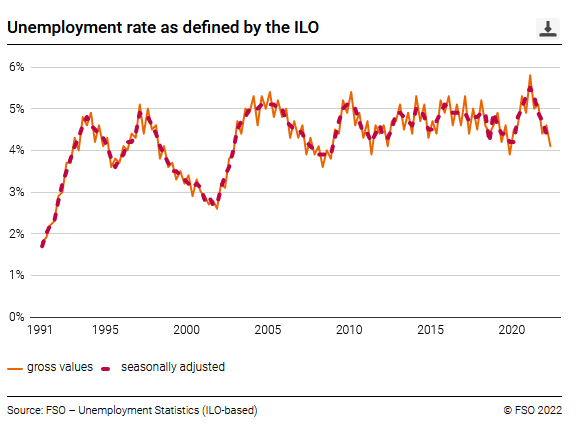
\includegraphics[width=0.8\textwidth]{ilo.png}
\end{center}
\footnotesize{Source: \href{https://www.bfs.admin.ch/bfs/en/home/statistics/work-income/unemployment-underemployment/ilo-unemployed.html}{\color{blue}Federal Statistical Office}}
\end{block}
}
\frame{
\begin{block}{Atmospheric CO2 on Mauna Loa, Hawaii}
\begin{center}
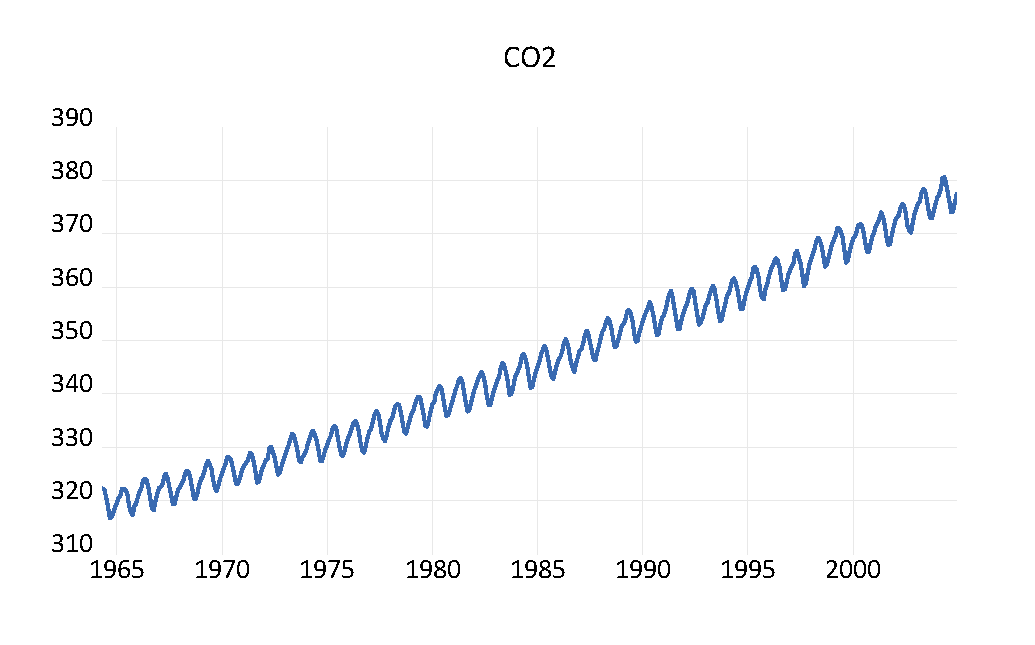
\includegraphics[width=0.8\textwidth]{co2}
\end{center}
\end{block}
}
\section{Descriptive TSA}
\frameit{Time Series Plots}{
\item The above plots were all examples of \er{time series plots}: plotting the data against time itself.
\item This is usually the first thing to do when looking at a new data set.
\item We'll see later how to make these plots.
}
\frameit{Decomposing a Time Series}{
\item The main tool of descriptive time series analysis it to decompose it into a \er{trend}, a \er{seasonal} component, and a \er{residual} component, according to the additive model
\[Y_t=F_t+S_t+U_t,\]
where the trend component $F_t$ models long-term movements, the seasonal component $S_t$ measures systematic seasonal patterns, and the residual component $U_t$ contains anything that cannot be explained by the other two\footnote{Sometimes economic time series also contain a cyclical component stemming from the business cycle, but we will ignore this here.}.
\item The Mauna Loa data make the trend and seasonal component very obvious.
}
\section{Trend Estimates}\subsection{OLS}
\frameit{Estimating a Linear Trend by OLS}{
\item One way to estimate a \er{linear trend} is to just regress the data on an intercept and time itself, i.e.,

\[
Y_t=\beta_0+\beta_1 t + U_t.
\]
\item The estimated trend is then
\[
\widehat{F_t} = \widehat{\beta_0}+\widehat{\beta_1} t.
\]
}
\frameit{Estimating a Quadratic Trend by OLS}{
\item As seen in the exercises, it is also possible to have a nonlinear trend. One example is a \er{quadratic} trend. This can be estimated via the regression

\[
Y_t=\beta_0+\beta_1 t +\beta_2t^2+ U_t.
\]
\item The estimated trend is then
\[
\widehat{F_t} = \widehat{\beta_0}+\widehat{\beta_1} t+\widehat{\beta_2} t^2.
\]
}
\frameit{Estimating an Exponential Trend by OLS}{
\item Another possibility is to use an \er{exponential} trend. The model is then
\[
F_t = \beta_0\cdot\beta_1^t.
\]
\item To estimate this by OLS, one takes logs:
\[
\log(F_t) = \log(\beta_0)+\log(\beta_1)\cdot t=:c+b\cdot t.
\]
\item Adding an error term, this exponential trend can be estimated via the regression
\[
\log(Y_t) = c+b\cdot t+U_t.
\]
\item The resulting trend function is
\[
F_t = \widehat{\beta_0}\cdot\widehat{\beta_1}^t, \quad\mbox{where } \widehat\beta_0=\exp(\hat{c}),\widehat\beta_1=\exp(\hat{b}).
\]
}
\frameit{Interpreting an Exponential Trend}{
\item If the trend is
\[
F_t = \beta_0\cdot\beta_1^t,
\]
then
\[
\frac{F_t}{F_{t-1}}=\frac{\beta_0\cdot\beta_1^t}{\beta_0\cdot\beta_1^{t-1}}=\beta_1;
\]
i.e., $Y_t$ grows by $100\cdot (\beta_1-1)$\% per period, on average.
\item Example $(\beta_0=1, \beta_1=1.05)$:
\[
F_t = 1.05^t,
\]
so $Y_t$ grows by 5\% a year, on average (cf. compounding interest).
}
\subsection{Moving Averages}
\frameit{Estimating the Trend via Moving Averages}{
\item Another approach, which has the advantage of adapting to the data automatically, rather than pre-specifying a functional form (linear, quadratic, exponential), is to estimate the trend via a \er{moving average.}
\item E.g., for a third-order moving average ($k=3$),
\[
\widehat{F_t}=(Y_{t-1}+Y_{t}+Y_{t+1})/3.
\]
\item Choice of $k$: the higher, the smoother. If seasonality is present, $k$ should cover at least a full cycle.
\item \er{Downside}: $(k+1)/2$ values at the end points cannot be computed. Thus also not useful for forecasting.
\item Note: for a moving average of even order, one averages $k+1$ data points, but the endpoints get half the weight. E.g., with $k=4$,
\[
\widehat{F_t}=\left(\frac{1}{2}Y_{t-2}+Y_{t-1}+Y_{t}+Y_{t+1}+\frac{1}{2}Y_{t+2}\right)/4.
\]
}

\section{Seasonality}\subsection*{bla}
\frameit{Dummy Variables}{
\item Simple way to address the seasonality $S_t$: \er{seasonal dummies}, which take the value one in one season, and zero in all others.
\item Example (see next page): say we have quarterly data. Then we would use four dummies, defined, for $j\in\{1,\ldots, 4\}$, as
\[d_{jt}=\begin{cases}1\mbox{, if observation $t$ is in season $j$,}\\0\mbox{, otherwise.} \end{cases}\]
\item Effectively, every season gets its own intercept.
\item Careful: if a full set of dummies is included, then the intercept must be left off, otherwise the regressors are perfectly collinear; this is the \er{dummy variable trap}.
\item Alternatively, keep the intercept, but remove one of the dummies. That season then becomes the baseline, and the other dummies measure the average difference from the baseline, per season.
}
\frame{
\begin{block}{Example}{
\begin{center}
\begin{tabular}{@{}llllll@{}}
\toprule
$t$ & Date   & $d_1$ & $d_2$ & $d_3$ & $d_4$ \\ \midrule
1 & 2021Q1 & 1    & 0    & 0    & 0    \\
2 & 2021Q2 & 0    & 1    & 0    & 0    \\
3 & 2021Q3 & 0    & 0    & 1    & 0    \\
4 & 2021Q4 & 0    & 0    & 0    & 1    \\
5 & 2022Q1 & 1    & 0    & 0    & 0    \\
6 & 2022Q2 & 0    & 1    & 0    & 0    \\
7 & 2022Q3 & 0    & 0    & 1    & 0    \\
8 & 2022Q4 & 0    & 0    & 0    & 1    \\
\vdots\\
 \bottomrule
\end{tabular}
\end{center}
}\end{block}
}
\frameit{Example continued}{
\item If we include a linear trend, then the model becomes
\begin{align*}
Y_t&=F_t+S_t+U_t\\
&=\beta_1\cdot t+\alpha_1d_{1,t}+\alpha_2d_{2,t}+\alpha_3d_{3,t}+\alpha_4d_{4,t}+U_t,
\end{align*}
which can be estimated by OLS.
\item If we want to produce a forecast for $Y_6$, which is in Season 2, then
\[
\widehat{Y_6}=\widehat{\beta_1}\cdot 6 + \widehat{\alpha_2}.
\]
}
\frameit{Example continued}{
\item Alternatively, include an intercept and drop one dummy:
\[
Y_t=\beta_0+\beta_1\cdot t+\alpha_1d_{1,t}+\alpha_2d_{2,t}+\alpha_3d_{3,t}+U_t.
\]
\item This makes Season 4 our baseline; the other seasons are measured in deviation from this baseline. 
\item The forecast for an observation in Season 4 is thus simply
\[
\widehat{Y_4}=\widehat{\beta_0}+\widehat{\beta_1}\cdot 4
\]
\item The other seasons are measured in deviation from the baseline; e.g., $\alpha_2$ is the average difference between Seasons 4 and 2:
\[
\widehat{Y_6}=\widehat{\beta_0}+\widehat{\beta_1}\cdot 6+\widehat{\alpha_2}.
\]

}
%\section{EWMA}\subsection*{bla}
%\frameit{Exponentially Weighted Moving Averages}{
%\item The problem that moving average cannot be computed at the boundaries, and hence not used for forecasting, can in principle be solved by using backward-looking, instead of centered, moving averages.
%\item Another problem remains though: the so-called \er{ghosting} problem. A data point (say an outlier) remains in the trend estimate for exactly $k$ periods, then suddenly drops out.
%\item Also, there is a \er{trade-off} in choosing $k$: larger values result in a smoother trend, but also make the trend react more slowly to changes.
%\item Solution: the \er{exponentially weighted moving average}, or \er{EWMA}.
%\item Idea: use \er{all} the data, but give more weight to recent observations.
%\item \er{Prerequisite}: trend and seasonality don't exist, or have been removed.
%}
\section{Epilogue}\subsection*{bla}
\frame{
\frametitle{Learning Goals}
Students
\begin{itemize}
\item Know the difference between cross-sectional and time series data,
\item know what a regular time series is, and what its frequency is,
\item are able to decompose a time series into trend, seasonality, and the residual component using Python,
\item and are able to produce time series plots in Python.
\end{itemize}
}
\frameit{Homework}{
\item Freshen up your statistics knowledge, if needed.
\item Exercise 1.
}
\end{document}
